\chapter{Natural Language Processing (NLP)}
Il \textbf{Natural Language Processing} (NLP) si occupa di studiare il linguaggio
naturale introducendo la semantica e le relazioni tra le parole. Oltre a questo,
si occupa di analizzare il testo, capire il contesto ed estrarre varie informazioni,
partendo dai topic fino ad arrivare alle emozioni.

In NLP la parte fondamentale è trovare una rappresentazione delle parole. Questo
non è una cosa banale in quanto:
\begin{itemize}
      \item Ci serve un contesto per rappresentare il testo in analisi.
      \item Ci può essere del rumore nei dati (dati errati o non fedeli).
      \item Può essere presente dell'ambiguità nelle frasi, per esempio abbiamo
            modi di dire. Questo viene risolto in diversi modi, ad esempio
            effettuando l'analisi sintattici, part-of-speech tagging, etc.
      \item Ambiguità sintattica, la quale viene risolta attraverso part-tree-disambiguation
\end{itemize}
I problemi legati all'ambiguità sono molto importanti in questo campo, e sono
studiati in modo approfondito. Per la loro risoluzione esistono diverse tecniche
che sono state sviluppate nel tempo e implementate in librerie.
Alcune di queste, forniscono sistemi per risolvere le ambiguità nelle frasi, i
quali si basano sulla costruzione di diversi alberi di parsing e restituiscono
l'albero della frase più probabile.

Tra le varie tipologie di ambiguità che possiamo incontrare distinguiamo due
tipologie:
\begin{itemize}
      \item Ambiguità emozionale: in una frase sono espresse emozioni contrastanti.
            Questo viene studiato attraverso la \textbf{sentiment analysis}.
      \item Ambiguità semantica: in una frase sono presenti parole che possono
            avere più significati. Questo viene studiato attraverso la
            \textbf{named-entity recognition} e in seguito il \textbf{named-entity
                  linking}.
\end{itemize}
\section{Sentiment analysis}
\begin{definizione}[\textbf{Text Analytics}]
      La \textbf{text analytics} è una tecnica che permette di estrarre informazioni
      dal linguaggio naturale per identificare informazioni soggettive e oggettive.
\end{definizione}
La fase di analisi consiste nel classificare il testo in base al fatto che esso
sia:
\begin{itemize}
      \item \textbf{Oggettivo}: si sta esprimendo un fatto.
      \item \textbf{Soggettivo} (emozione): si sta esprimendo un'emozione la quale
            può essere:
            \begin{itemize}
                  \item Positivo.
                  \item Negativo.
                  \item Neutrale: complesso perché spesso è molto vicino ad una
                        frase oggettiva o spesso si pesa la frase tra positiva e
                        negativa, quindi se è bilanciata è neutrale.
            \end{itemize}
\end{itemize}
Un'altra distinzione che possiamo fare è tra:
\begin{itemize}
      \item \textbf{Esplicito}: il testo esprime chiaramente un opinione.
      \item \textbf{Implicito}: il testo esprime un opinione in modo indiretto.
\end{itemize}
Un altro problema di riconoscere il sentiment è capire se nella frase è
presente dell'ironia o del sarcasmo.
\begin{definizione}
      Le emozioni sono un fenomeno psicologico che viene azionato da stimoli
      culturali oppure da esperienze passate. Esse possono essere:
      \begin{itemize}
            \item Rabbia
            \item Disgusto
            \item Paura
            \item Felicità
            \item Tristezza
            \item Sorpresa
      \end{itemize}
      Esiste una diversa classificazione, la quale le rappresenta con 8 emozioni
      graduali.
      \begin{figure}[!ht]
            \centering
            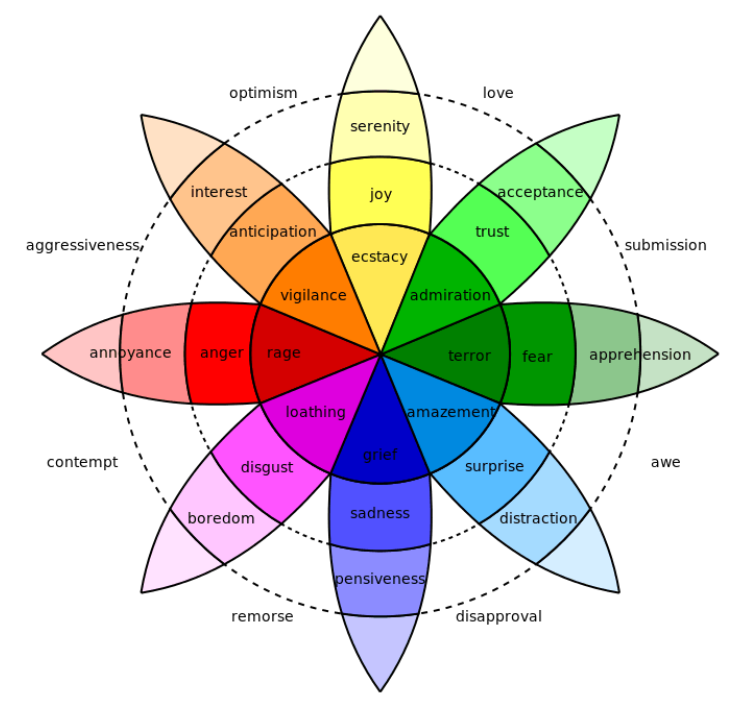
\includegraphics[width=0.5\textwidth]{./img/nlp/emozioni.png}
            \caption{Classificazione delle emozioni}
            \label{fig:emozioni}
      \end{figure}
\end{definizione}
\subsection{Rappresentazione del testo}
Il primo passo consiste nel capire come rappresentare il testo. Questo passaggio
è necessario per passare da una misura qualitativa a una misura quantitativa.

Una prima soluzione è quella di rappresentare il testo tramite un dizionario
di parole. Questo metodo è molto semplice e permette di rappresentare il testo
come un vettore di bit, dove il bit $i$-esimo è a $1$ se la parola $i$-esima
è presente nella frase. Questo metodo però ha dei problemi:
\begin{itemize}
      \item Il vettore che rappresenta la frase è molto grande e sparso.
      \item Perdiamo l'ordinamento delle parole.
\end{itemize}
Un ulteriore metodo è rappresentato dalla \textbf{BagOfWord}, la quale consiste
nel rappresentare una frase tramite un vettore in uno spazio. Il problema è che
manca la composizionalità delle parole.

Possiamo usare una rappresentazione deep basata su \textbf{word2vec}. Questa consiste
nello scrivere il termine sulla base dei termini che lo precedono e che lo seguono.
Si ha quindi uns strategia simile alla BagOfWord, ma mantenendo la composizionalità.

Word2Vec è un modello che viene usato per creare una rappresentazione vettoriale
delle parole. Questo modello è basato su una rete neurale che prende in input
una parola e cerca di prevedere le parole che la circondano.
\begin{itemize}
      \item \textbf{skip-gram}: parte da una parola del documento e cerca di
            predire l'intorno della parola.

            Per ottenere questo risultato, usiamo un \textbf{one-hot-vector},
            ovvero un bitvector, lungo quanto il il vocabolario, con un bit a $1$
            nella posizione associata alla parola all'interno del vocabolario.

            Successivamente costruiamo una rete neurale (Encoder Decoder) che
            preso in input il bitvector, in output dobbiamo avere un vettore
            lungo tanto quanto il vocabolario con una probabilità associata ad
            ogni parola. La rappresentazione vettoriale coincide con  quello che
            si ha nell'hidden layer, la sua dimensione è decisa in fase di
            costruzione della rete.

            Il documento viene rappresentato dal vettore media dei vettori dei
            termini presenti nel documento.

            A differenza dalle rappresentazioni più vecchie abbiamo un vettore di
            dimensione $n$ selezionato dalla rete. Il problema è che non consideriamo
            il contesto del mondo.

            Esistono metodi più efficaci per rappresentare il testo come
            \textbf{USE} e \textbf{BERT}.
      \item \textbf{CBOW}: cerca di predire la parola sulla base dell'intorno
            delle parole vicine.
\end{itemize}
Questi permettono di avere parole con lo stesso significato o simili vicine nello
spazio vettoriale.

Una volta risolto il problema della rappresentazione si può passare alla fase
di classificazione. Questa può essere fatta in diversi modi:
\begin{itemize}
      \item \textbf{Lexicon-based}: si basa su un dizionario di parole associate
            a delle emozioni. Si contano le parole associate alle emozioni e si
            restituisce l'emozione con il conteggio maggiore. Se le emozioni hanno
            lo stesso numero di parole allora la frase è neutra.
      \item \textbf{Machine Learning}: si basa su un modello di classificazione
            che prende in input il vettore che rappresenta la frase e restituisce
            l'emozione.
\end{itemize}
\begin{nota}
      Nel primo caso risulta importate scegliere bene il lessico, perché le parole
      possono essere positive o negative in base al contesto.
\end{nota}